\documentclass[14pt, aspectratio=169, handout]{beamer}
\usetheme{Copenhagen}
\usecolortheme{seahorse}
\setbeamertemplate{navigation symbols}{}
\setbeamertemplate{headline}{}

%\usepackage{pgfpages}
%\pgfpagesuselayout{4 on 1}[a4paper, border shrink=5mm]

\usepackage{graphicx} % Required for inserting images
\usepackage{multicol}
%\usepackage{enumitem}
\usepackage{amsfonts}
\usepackage{amsmath}
\usepackage{xcolor}
\definecolor{myblue}{RGB}{0, 0, 255} 
\definecolor{mygreen}{RGB}{0, 180, 80}
\definecolor{myred}{RGB}{153, 0, 0}
\definecolor{myorange}{RGB}{255, 153, 51}
\definecolor{mypurple}{RGB}{102, 0, 204}
\usepackage{tikz}

%--- commands for transform arrows----------------
\newcommand{\transform}[2]{%
    \begin{tikzpicture}
        % Open circle
        \draw[thick] (0,0) circle (0.1);
        % Line with number above and adjustable length
        \draw[thick] (0.1,0) -- (#2,0) node[midway, above] {#1};
        % Filled circle
        \filldraw[thick] (#2,0) circle (0.1);
    \end{tikzpicture}%
}
\newcommand{\invtransform}[2]{%
    \begin{tikzpicture}
        % filled circle
        \filldraw[thick] (0,0) circle (0.1);
        % Line with number above and adjustable length
        \draw[thick] (0.1,0) -- (#2 -0.1,0) node[midway, above] {#1};
        % open circle
        \draw[thick] (#2,0) circle (0.1);
    \end{tikzpicture}%
}
\newcommand{\verticaltransform}[4]{%
    \begin{tikzpicture}
        % Open circle at the bottom with text below
        \filldraw[thick] (0,0) circle (0.1) node[below=3pt] {$#4$};
        % Vertical line with number on the left
        \draw[thick] (0,0.1) -- (0,#2 -0.1) node[midway, left] {#1};
        % Filled circle at the top with text above
        \draw[thick] (0,#2) circle (0.1) node[above=3pt] {$#3$};
    \end{tikzpicture}%
}
\newcommand{\verticalinvtransform}[4]{%
    \begin{tikzpicture}
        % Open circle at the bottom with text below
        \draw[thick] (0,0) circle (0.1) node[below=3pt] {$#4$};
        % Vertical line with number on the left
        \draw[thick] (0,0.1) -- (0,#2) node[midway, left] {#1};
        % Filled circle at the top with text above
        \filldraw[thick] (0,#2) circle (0.1) node[above=3pt] {$#3$};
    \end{tikzpicture}%
}

\definecolor{darkblue}{RGB}{0, 0, 139}
\definecolor{lightblue}{RGB}{173, 216, 230}

\title{SST1 Übungsstunde 10}
\author{Matteo Dietz}
\date{December 2024}

\begin{document}

\maketitle

\begin{frame}{Themenüberblick}
    \begin{itemize}
        \item \textbf{$\mathcal{Z}$-Transformation}
        \item[] Definition, Konvergenzgebiete und Eigenschaften
        \item[] Zusammenhang zu Laplace Transformation und DTFT
        \item[] Anwendung auf zeitdiskrete LTI-Systeme
    \end{itemize}
\end{frame}

\begin{frame}{Aufgaben für diese Woche}
    \begin{itemize}
        \item[] \textbf{114}, \textbf{115}, 116 117 118, \textbf{119}, \textbf{120}, 121, \textbf{122}
        \item[] 
        \item[] Die \textbf{fettgedruckten} Übungen empfehle ich, weil sie wesentlich zu eurem Verständnis der Theorie beitragen und/oder sehr prüfungsrelevant sind.
    \end{itemize}
\end{frame}

\begin{frame}
{$\mathcal{Z}$-Transformation}
    \fcolorbox{darkblue}{lightblue}{%
    \parbox{\dimexpr\linewidth-2\fboxsep-2\fboxrule\relax}{
    \vspace*{0.15cm}
    $$\mathcal{Z}\{x[n]\} = X(z) = \sum_{n=-\infty}^\infty x[n]z^{-n}, \hspace{20pt} z \in \mathbb{C}$$
}}
\begin{itemize}
    \item[] 
    \item Die Summe $\sum_{n=-\infty}^\infty x[n]z^{-n}$ kann möglicherweise divergieren.
    \item[] 
    \item[] $\implies$ Wir müssen Konvergenzgebiete betrachten.
\end{itemize}

\end{frame}

\begin{frame}{Konvergenzgebiet (ROC)}
    \fcolorbox{darkblue}{lightblue}{%
    \parbox{\dimexpr\linewidth-2\fboxsep-2\fboxrule\relax}{
    \vspace*{0.15cm}
    $$\text{ROC}_X = \{z \in \mathbb{C} \; : \; X(z) \text{ konvergiert absolut}\}$$
}}%
\begin{itemize}
    \item $z= re^{2\pi i \theta} \implies \displaystyle\sum_{n=-\infty}^\infty \left| x[n]r^{-n}e^{-2\pi i n \theta} \right| = \displaystyle\sum_{n=-\infty}^\infty \left| x[n]r^{-n} \right|$
    \item[] $\implies$ ROC hängt nur von $|z|=r$ ab.
    \item[] $\implies$ ROC besteht aus Kreisscheiben um $z=0$:
    $$\text{ROC}_X = \{x \in \mathbb{C} \; : \; 0 \leq R_- < |z| < R_+ \leq \infty\}$$
    \item[] $\implies$ Konvergenzgebiet muss \textbf{zusammenhängend} sein.
\end{itemize}
\end{frame}

\begin{frame}{ROC: Rechtsseitige Signale}
    \begin{minipage}[t]{0.45\textwidth}
        \vspace*{0.25cm}
        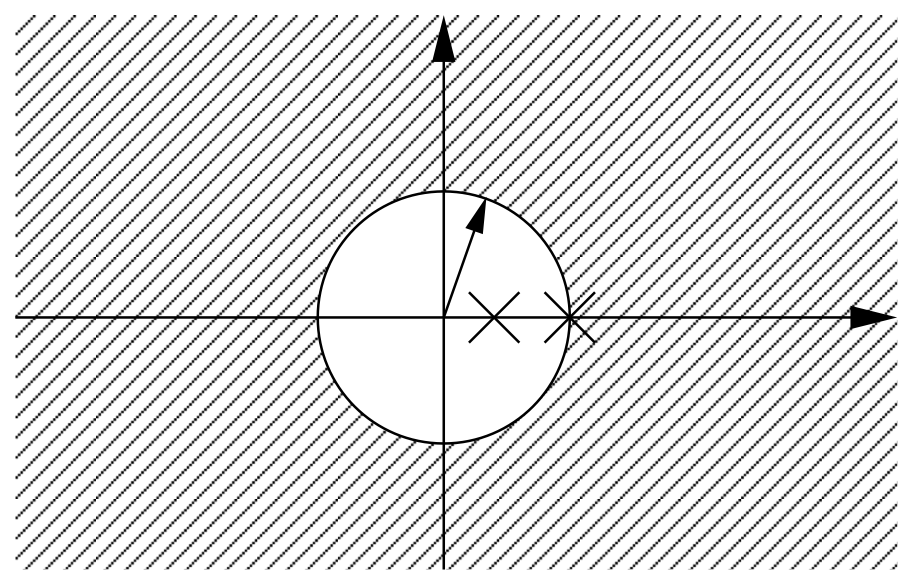
\includegraphics[width=\linewidth]{figures/Rechtsseitig.png}
    \end{minipage}
    \hfill
    \begin{minipage}[t]{0.45\textwidth}
        \vspace*{-0.75cm}
        $$X(z) = \sum_{n=N_1}^\infty x[n]z^{-n}$$
        $\mathcal{Z}$-Transformation $X(z)$ ist rational und $x[n]$ rechtsseitig $\implies$ ROC $=$ Region in der komplexen Ebene \textbf{ausserhalb des betragsweise grössten Poles} von $X(z)$ möglicherweise inklusive $|z|=\infty$.
    \end{minipage}
\end{frame}

\begin{frame}{ROC: Linksseitige Signale}
    \begin{minipage}[t]{0.45\textwidth}
        \vspace*{0.25cm}
        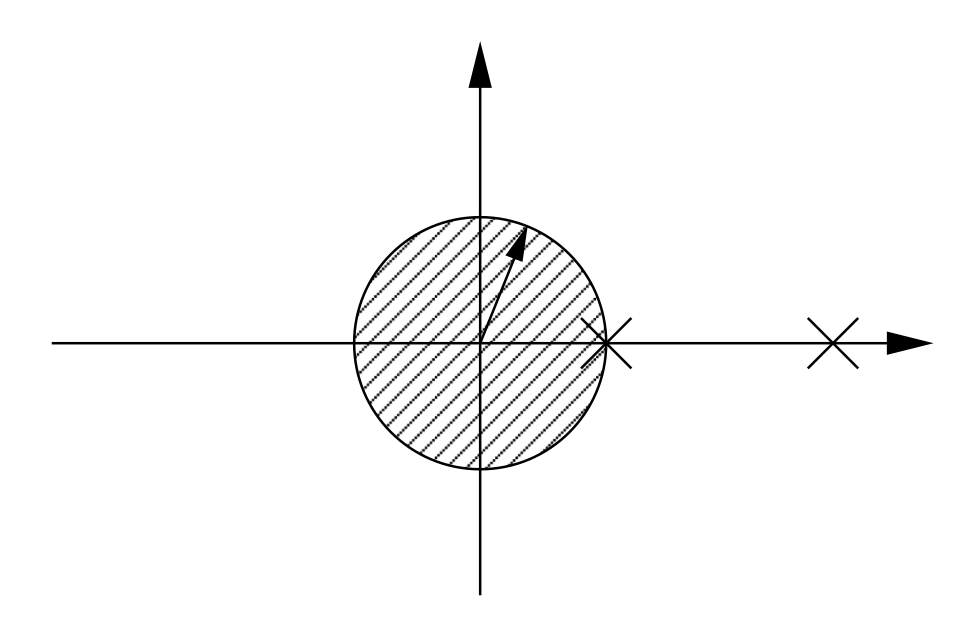
\includegraphics[width=\linewidth]{figures/Linksseitig.png}
    \end{minipage}
    \hfill
    \begin{minipage}[t]{0.45\textwidth}
        \vspace*{-0.75cm}
         $$X(z) = \sum_{k=-\infty}^M x[n]z^{-n}$$
         $\mathcal{Z}$-Transformation $X(z)$ ist rational und $x[n]$ linksseitig $\implies$ ROC $=$ Region in der komplexen Ebene \textbf{innerhalb des betragsweise kleinsten Poles} von $X(z)$ ausser möglicherweise $z=0$.
    \end{minipage}
\end{frame}

\begin{frame}{ROC: Beidseitige Signale}
    \begin{minipage}[t]{0.45\textwidth}
        \vspace*{0.1cm}
        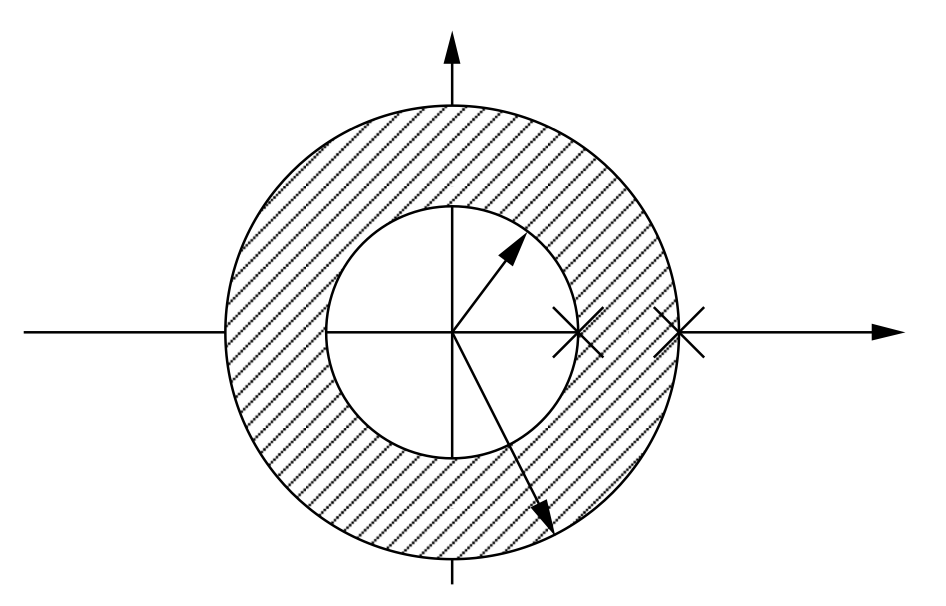
\includegraphics[width=\linewidth]{figures/Beidseitig.png}
    \end{minipage}
    \hfill
    \begin{minipage}[t]{0.45\textwidth}
        \vspace*{-0.5cm}
        Beidseitiges Signal $=$ Summe rechtsseitiges und linksseitiges Signal\\
        \vspace*{0.5cm}
        
        ROC enthält die Schnittmenge der ROCs vom rechtsseitigen und linksseitigen Signal.
    \end{minipage}
\end{frame}

\begin{frame}{ROC: Signale endlicher Länge}
    \begin{itemize}
        \item Ein Signal endlicher Länge nimmt nur an einer \textbf{endlichen Anzahl an Stellen} Werte ungleich null an.
        \item[] z.B. für $n$ mit $ -\infty < N \leq n \leq M <\infty $
        \item[] 
        \item $\mathcal{Z}$-Transformation ist die Summe einer endlichen Anzahl Terme und muss somit für $z\neq 0, \infty $ konvergieren, weil dann jeder Term der Summe endlich ist.
        \item[] 
        \item Die ROC kann aber muss nicht $z=0$ oder $\infty$ enthalten.
    \end{itemize}
\end{frame}

\begin{frame}{Aufgabe 115: ROCs}
    \begin{minipage}[t]{0.25\textwidth}
    a)\\
    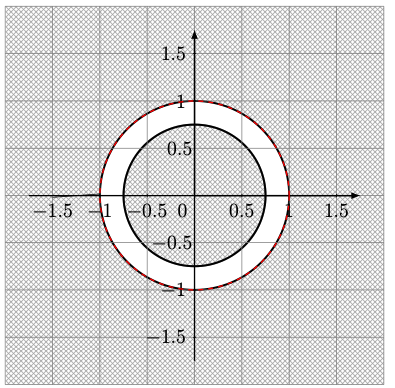
\includegraphics[width=\linewidth]{figures/a.png}
\end{minipage}
\hfill
\begin{minipage}[t]{0.25\textwidth}
    b)\\
    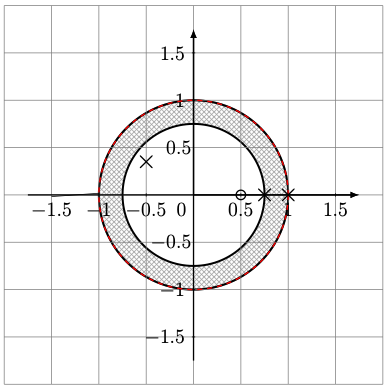
\includegraphics[width=\linewidth]{figures/b.png}
\end{minipage}
\hfill
\begin{minipage}[t]{0.25\textwidth}
    c)\\
    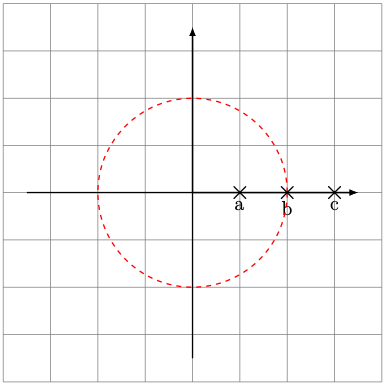
\includegraphics[width=\linewidth]{figures/c.png}
\end{minipage}
\end{frame}

\begin{frame}{Aufgabe 115: ROCs}
    \begin{minipage}[t]{0.25\textwidth}
    d.i)\\
    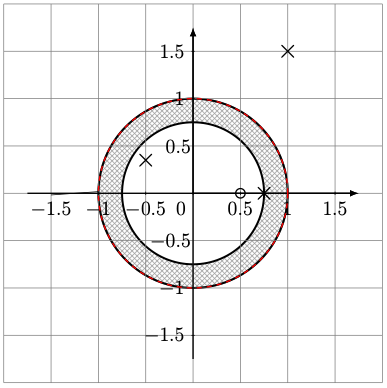
\includegraphics[width=\linewidth]{figures/di.png}
\end{minipage}
\hfill
\begin{minipage}[t]{0.25\textwidth}
    d.ii)\\
    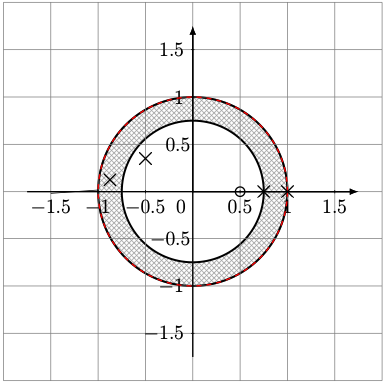
\includegraphics[width=\linewidth]{figures/dii.png}
\end{minipage}
\hfill
\begin{minipage}[t]{0.25\textwidth}
    d.iii)\\
    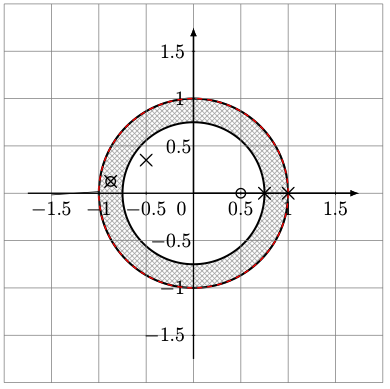
\includegraphics[width=\linewidth]{figures/diii.png}
\end{minipage}
\end{frame}

\begin{frame}{Eigenschaften der $\mathcal{Z}$-Transformation}
    \begin{itemize}
    \item \textbf{Linearität}:
        $$\mathcal{Z}\{ax[n] + by[n]\} = aX(z) + bY(z)$$ 
    \item[] Das Konvergenzgebiet ist mindestens ROC$_X \cap $ ROC$_Y$
    \item[] 
    \item \textbf{Zeitverschiebung}:
        $$\mathcal{Z}\{x[n-n_0]\} = z^{-n_0}X(z)$$
    \item[] Das Konvergenzgebiet bleibt gleich.
    \end{itemize}
\end{frame}

\begin{frame}{Eigenschaften der $\mathcal{Z}$-Transformation}
    \begin{itemize}
    \item \textbf{Faltung}:
        $$y[n] = (x \ast h)[n] \hspace{8pt} \transform{$\mathcal{Z}$}{1} \hspace{8pt} Y(z) = X(z)H(z) $$
    \item[] Das Konvergenzgebiet ist mindestens ROC$_X \cap $ ROC$_Y$
    \item[] 
    \item \textbf{Umkehrformel}:
        $$x[n] = \frac{1}{2 \pi i} \oint_C X(z)z^{n-1} \text{d}z$$
    \item[] $C=$ geschlossener Pfad in der ROC im Gegenuhrzeigersinn
    \end{itemize}
\end{frame}

\begin{frame}{$\mathcal{Z}$-Transformation: Formelsammlung}
    \begin{center}
        \vspace*{-0.34cm}
        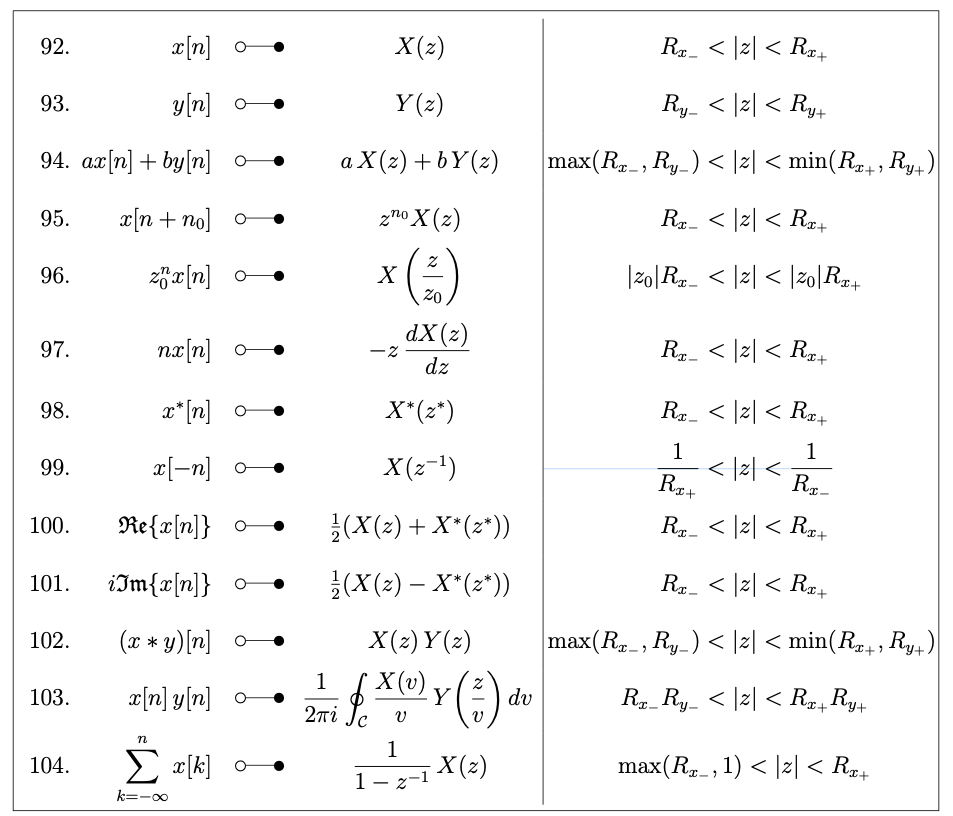
\includegraphics[width=0.63\linewidth]{figures/Z-Formelsammlung.png}
    \end{center}
\end{frame}

\begin{frame}{$\mathcal{Z}$-Transformation: Formelsammlung}
    \begin{center}
        \vspace*{-0.34cm}
        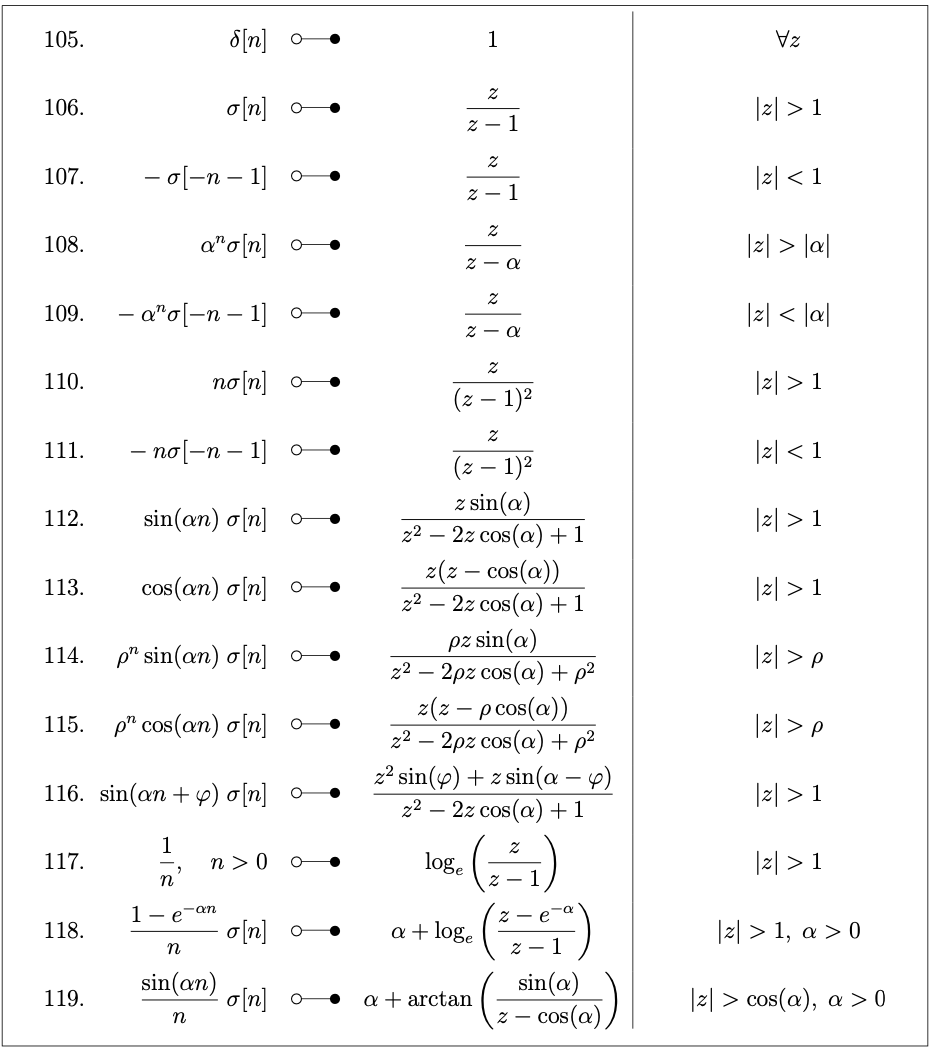
\includegraphics[width=0.48\linewidth]{figures/Z-Transformationspaare_pptx.png}
    \end{center}
\end{frame}

\begin{frame}{$\mathcal{Z}$-Transformation $\leftrightarrow$ Laplace-Transformation}
    \noindent

\begin{align*}
    &(\textbf{$\mathcal{Z}$-Transf.:}) \hspace{20pt} X(z) = \sum_{n=-\infty}^\infty x[n] z^{-n} \\
    &(\textbf{Laplace:}) \hspace{30pt} X(s) = \int_{-\infty}^\infty x(t) e^{-st} \text{d}t
\end{align*}

Die $\mathcal{Z}$-Transformation ist das zeitdiskrete Analogon zur Laplace-Transformation.
\end{frame}

\begin{frame}{$\mathcal{Z}$-Transformation $\leftrightarrow$ DTFT}
    \begin{align*}
        &(\textbf{$\mathcal{Z}$-Transf.:}) \hspace{20pt} X(z) = \sum_{n=-\infty}^\infty x[n] z^{-n} \\
        &(\textbf{DTFT:}) \hspace{40pt} \hat{x}(\theta) = \sum_{n=-\infty}^\infty x[n] e^{-2 \pi i n \theta} 
    \end{align*}

    Die DTFT ist die $\mathcal{Z}$-Transformation \textbf{ausgewertet auf dem Einheitskreis} in der komplexen Ebene
\end{frame}

\begin{frame}{Aufgabe 122: $\mathcal{Z}$-Transformation $\leftrightarrow$ DTFT}
    Es sei $x[n] = \delta[n+3] + \delta[n-3]$
\begin{itemize}
    \item[a)] Berechnen Sie die $\mathcal{Z}$-Transformierte $X(z)$ von $x[n]$.
    \item[b)] Schliessen Sie aus dem Ergebnis in a) auf die zeitdiskrete Fouriertransformierte $\hat{x}(\theta)$ von $x[n]$.
    \item[c)] Berechnen Sie den Betrag und die Phase von $\hat{x}(\theta)$.
    \item[]
    \item[] 
    \item[]
    \item[]
    \item[]
    \item[] 
\end{itemize}
\end{frame}

\begin{frame}{Anwendungen $\mathcal{Z}$-Transformation auf LTI-Systeme}
    $$\sum_{k=0}^N a_k y[n-k] = \sum_{m=0}^M b_m x[n-m]$$ \vspace*{-0.5cm}$$ \verticaltransform{95.}{1}{}{} \hspace{28pt}$$ \vspace*{-1.25cm}$$\left( \sum_{k=0}^N a_k z^{-k} \right)Y(z) = \left( \sum_{m=0}^M b_m z^{-m} \right)X(z) $$
    \vspace*{0.5cm}$$H(z) = \frac{Y(z)}{X(z)} = \frac{\sum_{m=0}^M b_m z^{-m}}{\sum_{k=0}^N a_k z^{-k}}$$
\end{frame}

\begin{frame}{Kausalität}
   Das LTI-System ist kausal, falls $h[n]$ \textbf{rechtsseitig} ist, d.h. wenn ROC$_H$ ausserhalb der betragsweise grössten Poles liegt.
   
            \begin{center}
            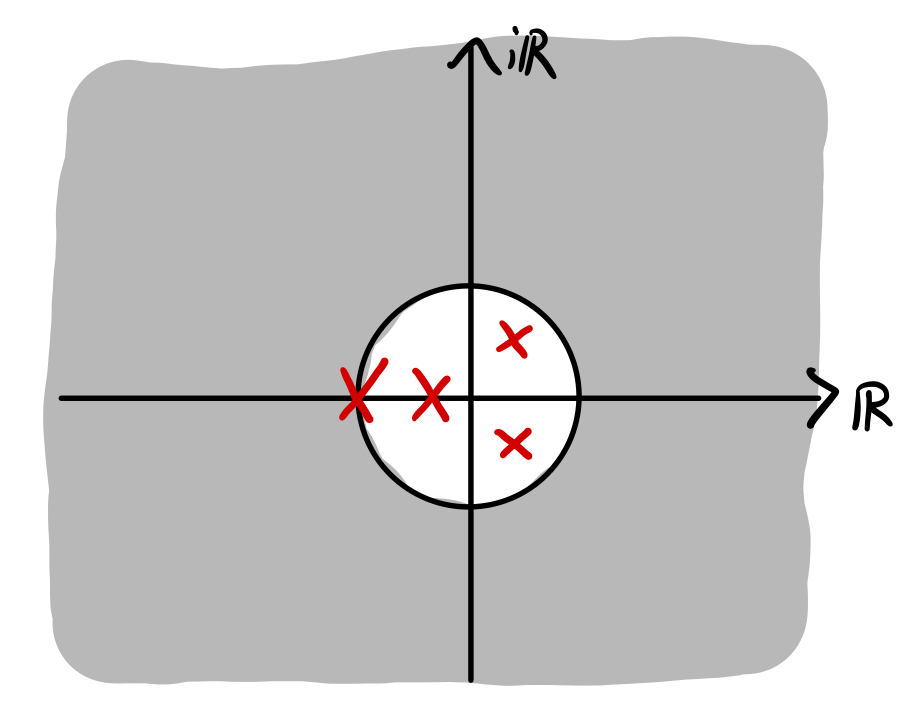
\includegraphics[width=0.4\linewidth]{figures/kausal.jpg}
        \end{center}
\end{frame}

\begin{frame}{BIBO-Stabilität}
    $$\sum_{n=-\infty}^\infty |h[n]| < \infty \Leftrightarrow \sum_{n=-\infty}^\infty |h[n]z^{-n}| < \infty \text{ mit } |z|=1$$
    \begin{itemize}
        \item[] LTI-System BIBO-stabil, falls \textbf{Einheitskreis $\subseteq$ ROC}$_H$ liegt, d.h. wenn $\{ z \in \mathbb{C} \; : \; |z| = 1 \} \subseteq \text{ROC}_H$. 
        \item[] Wenn $H(z)$ rational ist, ist es eine Äquivalenz.
    \end{itemize}
    \begin{center}
        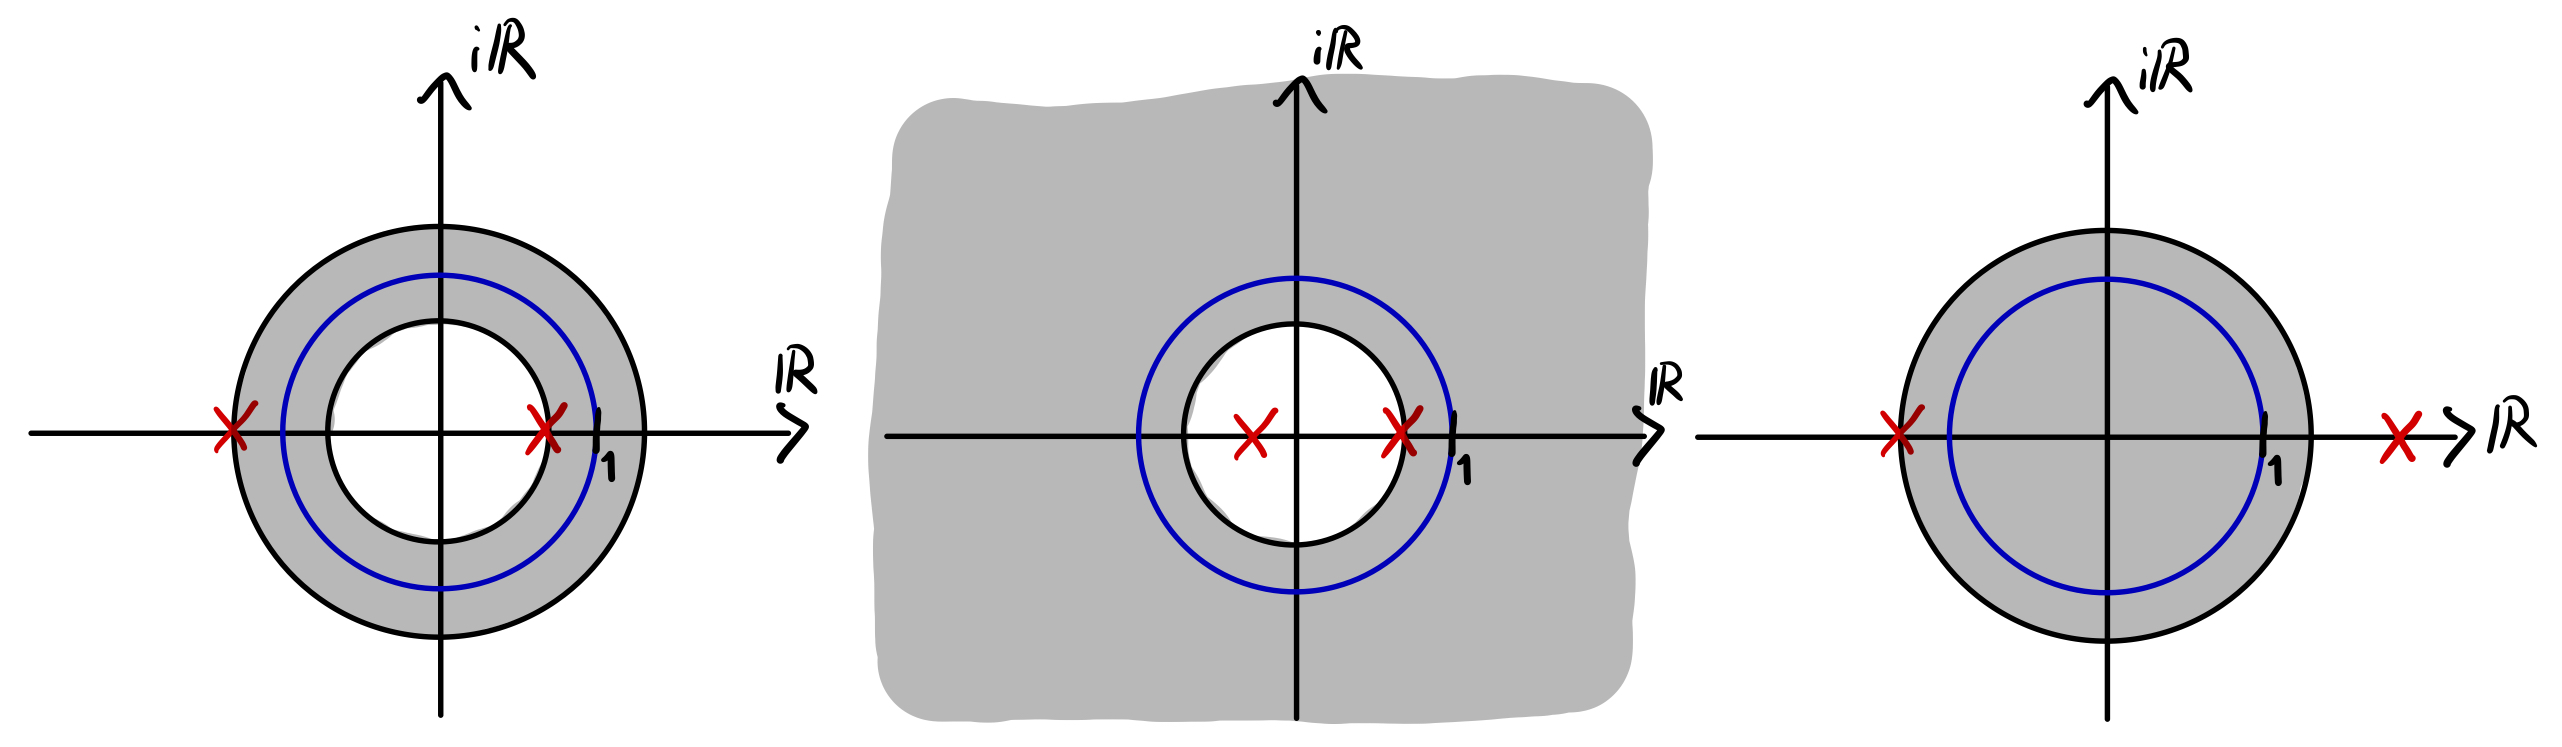
\includegraphics[width=0.75\linewidth]{figures/BIBO_stabil.jpg}
    \end{center}
\end{frame}

\begin{frame}{Serien- und Parallelschaltung von LTI-Systemen}
    \begin{minipage}[t]{0.45\textwidth}
            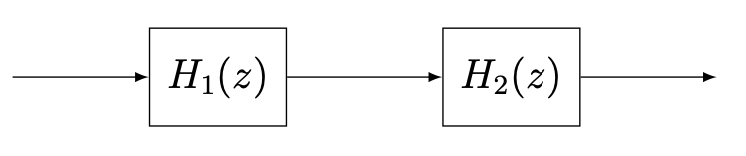
\includegraphics[width=\linewidth]{figures/Serienschaltung.png}
            \end{minipage}
            \hfill
            \begin{minipage}[c]{0.45\textwidth}
            $$H(z) = H_1(z)H_2(z)$$
            \vspace*{0.77cm}
            \end{minipage}

            \begin{minipage}[t]{0.45\textwidth}
            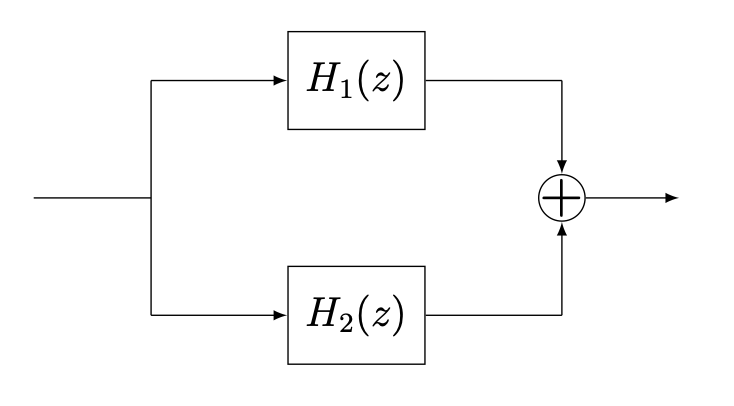
\includegraphics[width=\linewidth]{figures/Parallelschaltung.png}
            \end{minipage}
            \hfill
            \begin{minipage}[c]{0.45\textwidth}
            $$H(z) = H_1(z) + H_2(z)$$
            \vspace*{3.45cm}
            \end{minipage}
            \vspace*{-3.5cm}
\end{frame}

\begin{frame}{Rückkopplung}
        \begin{minipage}[t]{0.45\textwidth}
            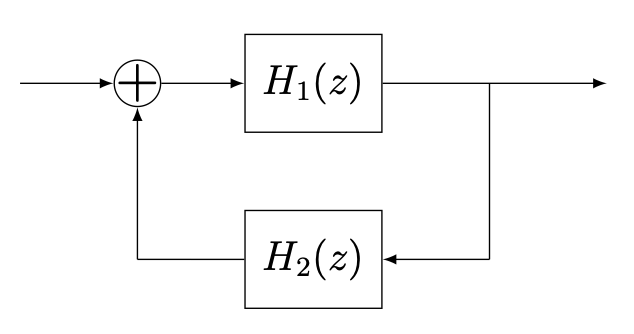
\includegraphics[width=\linewidth]{figures/Rueckkopplung.png}
        \end{minipage}
        \hfill
        \begin{minipage}[c]{0.45\textwidth}
            \small{
            \begin{align*}
                &X(z)H_1(z) + H_2(z)Y(z)H_1(z) = Y(z) \\
                &X(z)H_1(z) = Y(z)(1-H_1(z)H_2(z)) \\
                &H(z)=\frac{H_1(z)}{1-H_1(z)H_2(z)}
            \end{align*}}
            \vspace*{3.45cm}
        \end{minipage}
        \vspace*{-3.5cm}
\end{frame}

\begin{frame}{Prüfungsaufgabe: Frühjahr 2024, Aufgabe 3}
    
\end{frame}

\end{document}
